\chapter{Discussion}

\label{ch:conc}

\epigraph{\textit{These thoughts are constructive criticisms. Pyramidical. I try to suppress these thoughts, but they leak out...}}{George Saden -- \textit{Zardoz}}

\vspace{1cm}

\par\noindent In Chapters \ref{ch:IGR} and \ref{ch:BPbig} I discuss new ways of classifying variability\index{Variability} in the unusual LMXB\index{X-ray binary!Low mass}s IGR J17091\index{IGR J17091-3624} and the Bursting Pulsar\index{Bursting Pulsar}.  I use the new classification frameworks I have created to compare these objects with the similar LMXBs GRS 1915\index{GRS 1915+105} and the Rapid Burster\index{Rapid Burster}.  While I find a number of similarities between these objects, I also highlight a number of differences.  For example, I find that the spectral\index{Spectroscopy} evolution during variability in IGR J17091 is very different to in GRS 1915, and the bursts\index{X-ray burst} in the Bursting Pulsar evolve in a very different way to those seen from the Rapid Burster.
\par A common theme throughout the work presented in this thesis is that the variability\index{Variability} in these unusual objects is even more complex than had previously been thought.  Application of Occam's razor\index{Occam's razor} \citep{Occam} suggests that the similar variability from these objects is generated by similar physics, but I have found that it is difficult to unify the diverse behaviours of these unusual systems.  I also compare the four objects that I focus on with other unusual XRBs\index{X-ray binary} such as Terzan 5 X-2\index{Terzan 5 X-2} and, in Chapter \ref{ch:BPletter}, TMSPs\index{TMSP}.  In this chapter I further discuss the relationships between these seemingly disparate objects, and how my findings fit in to the more general picture of accretion\index{Accretion} in these extreme and bizarre systems.

\section{General Observations}

\label{sec:disccomp}

\subsection{Variability Evolution throughout an Ouburst}

\par One feature common to at least 3\footnote{As GRS 1915\index{GRS 1915+105} has been in outburst\index{Outburst} since its discovery, it is unknown how its variability classes\index{Variability class} vary over the duration of an outburst.} of the unusual LMXBs\index{X-ray binary!Low mass} discussed in this thesis is that variability\index{Variability} changes in a predictable way over the course of an outburst.  This effect is most apparent in the results I present in Chapter \ref{ch:BPbig}, where I discuss an evolution of bursting\index{X-ray burst} which is observed in both the 1996 and 1997 outbursts of the Bursting Pulsar\index{Bursting Pulsar}:
\begin{itemize}
\item Normal Bursts\index{Normal burst} and Minibursts\index{Miniburst} begin to occur shortly after the peak of each outburst.
\item Bursting shuts off entirely when the persistent intensity\index{Persistent emission} of the source decreases below $\sim0.1$\,Crab.
\item The persistent flux of the system increases in a rebrightening\index{Re-flare} event, at which point Mesobursts\index{Mesoburst} begin to occur.
\item Mesobursts evolve into Structured Bursting\index{Structured bursting}.
\end{itemize}
\par A predictable evolution of variability\index{Variability} throughout an outburst\index{Outburst} has also been identified in the Rapid Burster\index{Rapid Burster} (e.g. \citealp{Bagnoli_PopStudy}).  In this system, Type II\index{X-ray burst!Type II} bursts near the start of each outburst are Eddington\index{Eddington limit}-Limited and persist for $\sim100$s of seconds (see e.g. the upper panel of Figure \ref{fig:bagnoli_lcs}).  As the outburst evolves, these bursts become shorter, fainter and more sharply peaked (see e.g. the lower panel of Figure \ref{fig:bagnoli_lcs}).  This evolution is qualitatively very different from the evolution of variability seen in the Bursting Pulsar\index{Bursting Pulsar}.  However, the fact that bursting in both objects changes in a predictable way throughout each outburst shows that bursting in both objects is dependent on the accretion rate\index{Accretion rate} in the system and on the state of its accretion disk\index{Accretion disk}.
\par There is also some evidence of an evolution of the variability\index{Variability} displayed by IGR J17091\index{IGR J17091-3624}.  In Figure \ref{fig:WhereCls} I show a number of lightcurves\index{Lightcurve} of the 2011 outburst\index{Outburst} of IGR J17091\index{IGR J17091-3624}, highlighting when in the outburst each of our 9 variability classes\index{Variability class} was observed.  Although the evolution between classes apparently not as strict as in the Bursting Pulsar\index{Bursting Pulsar}, it is easy to identify a number of patterns in the data, such as:
\begin{itemize}
\item Class I\indexi\footnote{See Section \ref{sec:IGRclassesintro} for a description of each class.} only occurs near the start of the outburst\index{Outburst}, within 25 days of the onset of variability\index{Variability}.
\item Class II\indexii\ only occurs during two dips\index{Dip} in the persistent flux\index{Persistent emission} to a level of $\sim20$\,mCrab.
\item Class VII\indexvii\ only occurs while the persistent flux\index{Persistent emission} of IGR J17091\index{IGR J17091-3624} is in a narrow band centred on $\sim70$\,mCrab.
\end{itemize}
It is unclear whether a similar evolution occurs during the 2016 outburst\index{Outburst} of IGR J17091\index{IGR J17091-3624}, as a variability\index{Variability} population study\index{Population study} for this outburst has not yet been performed.  However these results from the 2011 outburst suggest that variability in IGR J17091 also depends strongly on the accretion rate\index{Accretion rate} and the state of the disk\index{Accretion disk}, as it is in the Rapid Burster\index{Rapid Burster} and the Bursting Pulsar\index{Bursting Pulsar}, and therefore variability should evolve in a predictable way over the course of each outburst.

\subsection{Criteria for Exotic Variability}

\label{sec:criteria}

\par As we show in Figure \ref{fig:IGR2016}, the 2016 outburst of IGR J17091 displayed similar variability to that which it showed in 2011 (e.g. \citealp{Reynolds_2016HB}), meaning that variability was not unique to the source's 2011 outburst.  Additionally Type II bursting has been seen in the 1996, 1997 and 2014 outbursts of the Bursting Pulsar, and the Rapid Burster goes into outburst regularly every $\sim$100--200 days and always displays Type II bursts.  Therefore 3 of the 4 objects I discuss in this thesis have produced their characteristic variable behaviour during multiple separate outbursts\footnote{As GRS 1915 has been in outburst since discovery, it is not possible to tell whether its variability is repeated in subsequent outbursts.}.  This observation strongly suggests that the ability to produce such variability is a property of the system rather than of an individual outburst.  In these systems some set of parameters, which persist between outbursts, are just right to allow these exotic types of variability to occur.

\begin{figure}
  \centering
  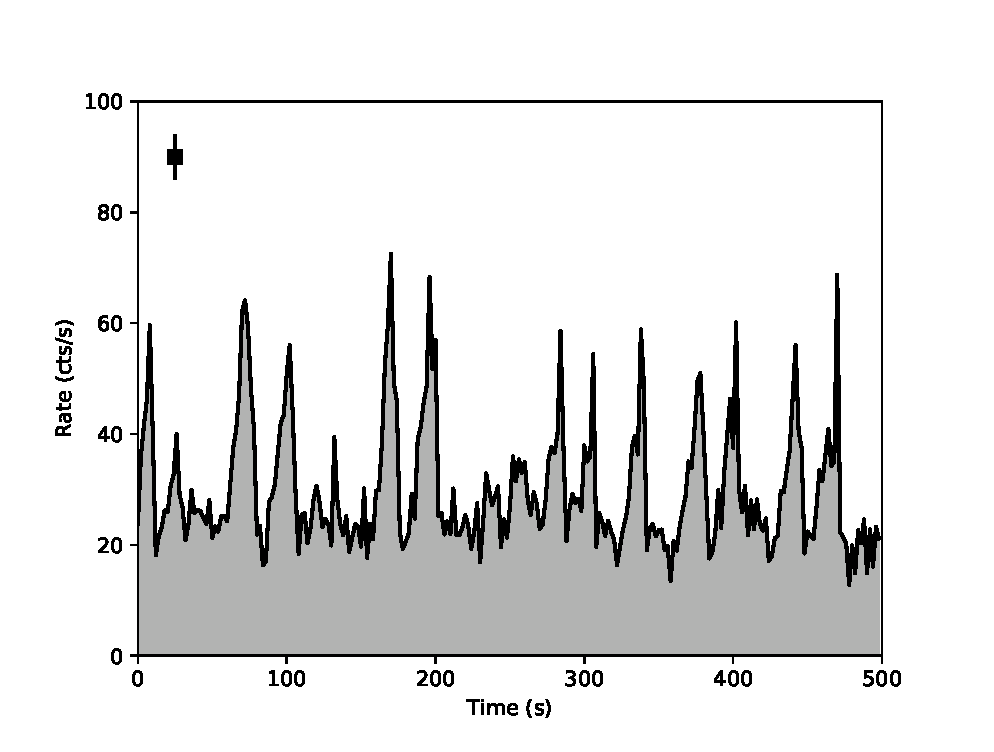
\includegraphics[width=.9\linewidth, trim= 0mm 0mm 10mm 10mm,clip]{images/new16plot.eps}
  \caption[A \textit{Swift}/XRT lightcurve of IGR J17091-3624 during its 2016 outburst, showing Class III variability.]{0.3--10\,keV \indexxrt\textit{Swift}/XRT lightcurve\index{Lightcurve} of IGR J17091-3624\index{IGR J17091-3624} during its 2016 outburst\index{Outburst}.  The black bar shows the typical size of errors.  This lightcurve shows Class III\indexiii\ variability\index{Variability}, which I identify in the 2011 outburst of this source and describe in Section \ref{sec:classIII}.}
  \label{fig:IGR2016}
\end{figure}

\par Compact objects\index{Compact object} are relatively simple, and they can be well-defined with only a few parameters:

\begin{itemize}
\item The type of compact object\index{Compact object} (neutron star\index{Neutron star} or black hole\index{Black hole}).
\item Mass.
\item Spin\index{Spin} and rate of change of spin.
\item Radius.
\item Magnetic Field\index{Magnetic field} Strength.
\end{itemize}

Where the last two parameters only apply if the object is a neutron star\index{Neutron star}.  In addition to these, one only has to describe the companion star\index{Companion star} (mass, mass loss rate, spectral type etc.), the parameters of the system orbit (eccentricity, semi-major axis, inclination and misalignment from the spin axes of both stars) and the mass transfer rate to fully describe an LMXB\index{X-ray binary!Low mass} system.  Due to this relative simplicity, there are not many candidates for parameters which govern the existence of exotic variability\index{Variability}.
\par GRS 1915+105\index{GRS 1915+105} contains the highest mass black hole\index{Black hole} confirmed in an LMXB\index{X-ray binary!Low mass}\footnote{At least one HMXB\index{X-ray binary!High mass}, Cyg X-1\index{Cyg X-1}, is believed to contain a black hole with higher mass \citep{Orosz_CygX1}.} ($12.4\pm2.0$\,M$_\odot$, \citealp{Reid_Parallax}), although many other LMXBs are believed to contain black holes\index{Black hole} with comparable masses (e.g. V404 Cyg\index{V404 Cyg}, \citealp{Shahbaz_V404}).  The black hole in GRS 1915 also has a very high spin\index{Spin}, with a spin\index{Spin} parameter of $0.98\pm0.01$ \citep{Miller_GRSspin}, but a number of other XRBs\index{X-ray binary} are also believed to harbour near-maximal spin black holes (see e.g. \citealp{Fragos_spin}).  Therefore it seems unlikely that mass or spin alone provide the criteria for GRS 1915-like variability\index{Variability}.%  In Chapter \ref{ch:BPletter} we consider a `hiccup'-like accretion behaviour as a possible mechanism behind variability in the Bursting Pulsar; this mechanism relies on specific ranges for the values of spin and magnetic field strength, but cannot be used to explain any of the variability seen in black hole systems.
\par Lense-Thirring precession\index{Lense-Thirring precession} in the disk\index{Accretion disk}, a frame-dragging effect\index{Frame-dragging} caused by the misalignment of the orbital and spin\index{Spin} axes of the compact object\index{Compact object}, has been used to explain some of the variability\index{Variability} seen in LMXBs\index{X-ray binary!Low mass} (e.g. \citealp{Stella_LT}).  However, the timescale of the variability\index{Variability} this generates is no slower than $\sim0.1$\,s \citep{Ingram_Solid}, too fast to be linked with the $\lesssim0.1$\,Hz variability seen from GRS 1915\index{GRS 1915+105}.  Instead the other parameters on the list, or a combination thereof, must be the determining factors in whether or not an object can display exotic variability.
%\par While I find that Eddington-limited accretion is not necessary for either GRS 1915-like variability or Type II bursting, all of the objects considered in this thesis have relatively high accretion rates during the peak of their outbursts: the Rapid Burster, which is likely the least luminous of the four systems, accretes at $\sim20$\% of its Eddington rate at peak.  While a high accretion rate is obviously not sufficient for GRS 1915-like variability or Type II bursting to occur, as many systems with high accretion rates do not display either behaviour, this result suggests that a high accretion rate may be a necessary criterion.
\par GRS 1915\index{GRS 1915+105} has a very long orbital period\index{Orbital period} of $\sim30$ days \citep{Neil_GRSPeriod}, and this is believed to result in it having the largest accretion disk\index{Accretion disk} of all known X-ray binaries\index{X-ray binary}.  This likely explains how GRS 1915 has been in outburst\index{Outburst} for such a long period of time ($\gtrsim20$ years, compared to the $\lesssim2$\,year outbursts\index{Outburst} seen in most black hole\index{Black hole} LMXB\index{X-ray binary!Low mass}s).  The orbital periods of IGR J17091\index{IGR J17091-3624} and the Rapid Burster\index{Rapid Burster} are unknown, but the Bursting Pulsar\index{Bursting Pulsar} also has a relatively long orbital period of 11.8 days (e.g. \citealp{Finger_BP}), suggesting that a large disk\index{Accretion disk} may also be a factor in the generation of exotic variability\index{Variability}.
\par Another property to consider is the magnetic field\index{Magnetic field} strength in the disk\index{Accretion disk}.  Although astrophysical black holes\index{Black hole} do not have a magnetic field, magnetic fields in a black hole can still arise from one of two sources:
\begin{itemize}
\item The field of the system's donor star\index{Companion star}, including field lines advected into the disk by accretion\index{Accretion}.
\item The movement of ionised material within the disk\index{Accretion disk}.
\end{itemize}
The presence of such a magnetic field\index{Magnetic field} may be able to stabilise an accretion disk\index{Accretion disk} against the instabilities\index{Instability} described in Section \ref{sec:diskinstab} (e.g. \citealp{Sadowski_MagField}.  \citeauthor{Sadowski_MagField} calculates the minimum magnetic field strength which, when threaded through a radiation-dominated\index{Radiation pressure} disk undergoing the instability described by \citet{Shakura_Instab}, would be able to stabilise the disk.  Assuming that such a field in an LMXB\index{X-ray binary!Low mass} is provided by the companion star\index{Companion star}, they find that this minimum value in an LMXB depends mostly on the luminosity of the system and the mass of the compact object\index{Compact object}.  They estimate the value of the minimum stabilising field strength in a number of black hole X-ray binaries, and find that the field required to stabilise GRS 1915\index{GRS 1915+105} is $\sim5.7\times10^{23}$\,G\,cm$^2$; this is over twice as large as the second highest value they find for an LMXB ($1.9\times10^{23}$\,G\,cm$^2$ for XTE J1550-564\index{XTE J1550-564}).  This high value is due to the large black hole\index{Black hole} mass in GRS 1915, and the fact that this black hole accretes at a near-Eddington\index{Eddington limit} rate\index{Accretion rate} and, thus, a high luminosity.  In this picture, therefore, GRS 1915-like variability may simply be a manifestation of the \citet{Shakura_Instab} instability which is suppressed in most LMXBs.  One could test the viability of this scenario by calculating the minimum stabilising field for IGR J17091\index{IGR J17091-3624}.  Unfortunately at time of writing the companion star to IGR J17091 has not been conclusively identified, and the mass and distance (and hence luminosity) of the system remain poorly constrained.
\par It is worth noting that the scenario suggested by \citet{Sadowski_MagField} by itself is unable to account for Type II\index{X-ray burst!Type II} bursts as, in these systems, the neutron star\index{Neutron star} is able to provide more than enough magnetic\index{Magnetic field} flux to stabilise the inner disk\index{Accretion disk} in the scenario of \citeauthor{Sadowski_MagField}.  However, the scenario of \citeauthor{Sadowski_MagField} does not take into account the effects of the magnetic disruption of the inner disk, nor does it account for any effects caused by the disk's interaction with the rapidly spinning neutron star magnetic field.

\subsection{Evidence of System Memory}

\par Another notable observation from these objects is that variability\index{Variability} in both GRS 1915\index{GRS 1915+105} and IGR J17091\index{IGR J17091-3624} falls into a discrete set of variability classes\index{Variability class}.  In both objects, a variability class could be observed on one day, not be observed for weeks and then reappear in a later observation.  Somehow, the physics that governs variability in these systems only permit the system to occupy one of a discrete set of variability classes.  In Figure \ref{fig:IGR2016} I show evidence that at least one of the variability classes I identified in the 2011 outburst\index{Outburst} of IGR J17091 occurred again in 2016.  This suggests that GRS 1915-like systems are somehow able to `remember' which variability classes they can occupy, and that this memory persists between outbursts.  This in turn means that, in addition to determining whether or not GRS 1915-like variability can occur, the simple parameters that define a black hole\index{Black hole} LMXB\index{X-ray binary!Low mass} also determine \textit{which} classes of GRS 1915-like variability can occur.
\par In Section \ref{sec:IGRcomp}, I report that two of the classes\index{Variability class} of variability I find in IGR J17091\index{IGR J17091-3624} (Classes VII\indexvii\ and VIII\indexviii) are unlike anything which has ever been seen in GRS 1915\index{GRS 1915+105} (see also Table \ref{tab:class_assign}).  This leads to one of three possibilities:
\begin{itemize}
\item Class VII\indexvii\ and VIII\indexviii-like variability has occurred in GRS 1915\index{GRS 1915+105} since its discovery, but coincidentally we have never observed it.  As GRS 1915 has been observed extensively during its ongoing $\gtrsim20$ year-long outburst\index{Outburst}, this is unlikely to be true.
\item Class VII and VIII variability preferentially occurs during a specific disk\index{Accretion disk} configuration which occurs at a specific point in the evolution of an outburst, and GRS 1915 is not currently in this state.
\item Some set of system parameters in IGR J17091\index{IGR J17091-3624} are different from in GRS 1915 in such a way that many variability classes\index{Variability class} can appear in both objects, but a small set of different variability classes are permitted in each object.
\end{itemize}
\par The final possibility is of great interest.  Future observations of IGR J17091\index{IGR J17091-3624} will aim to better constrain the parameters that define the system.  If these parameters are then compared to the already well-constrained parameters of GRS 1915\index{GRS 1915+105}, then we may be able to learn exactly which physical properties of the system govern which set of variability classes\index{Variability class} can be displayed.
\par There is also evidence of some degree of system memory in the Type II\index{X-ray burst!Type II} bursting systems.  The near-identical evolutions of variability\index{Variability} in the 1996 and 1997 outbursts\index{Outburst} of the Bursting Pulsar\index{Bursting Pulsar} indicate that the factors governing this evolution persist between outbursts in this object as well.
\par The Normal Bursts\index{Normal burst} and Minibursts\index{Miniburst} of the Bursting Pulsar\index{Bursting Pulsar}, which I describe in Sections \ref{sec:Normal_Bursts} and \ref{sec:Minibursts} respectively, also provide evidence of system memory in the Bursting Pulsar.  Both types of burst\index{X-ray burst} display a number of similar features and they occur interchangeably during the same period of each outburst\index{Outburst}, leading to the possibility that they are generated by the same physical instability\index{Instability}.  As I show in Figure \ref{fig:minidips}, Minibursts and Normal Bursts fall into two clear populations\index{Population study} when plotted by their amplitudes: we find no Normal or Minibursts with fluences between $\sim10^4$ and $\sim10^5$ 2--60\,keV PCA\indexpca\ counts.  Due to the large number of Minibursts and Normal Bursts observed in my study, it is highly likely that this gap is real.  Observations of future outbursts of the Bursting Pulsar will allow us to see whether this fluence gap always spans the same range, or whether this gap changes between outbursts as a function of the longer-term evolution of the system.

\section{IGR J17091 vs. the Bursting Pulsar: A Comparison}

\par It is clear that there are a number of significant similarities between objects which display Type II\index{X-ray burst!Type II} bursts and GRS 1915\index{GRS 1915+105}-like variability\index{Variability}.  What remains unclear is how, if at all, the physics of GRS 1915-like variability and Type II bursting are related to each other.  Many of the models proposed to explain GRS 1915-like variability and Type II bursts rely on similar viscous\index{Viscosity} disk instabilities\index{Instability} (see Sections \ref{sec:models_GRS} and \ref{sec:TIImod}), and the discovery of GRS 1915-like patterns in lightcurves\index{Lightcurve} of the Rapid Burster\index{Rapid Burster} strongly suggests a link between these two classes of object \citep{Bagnoli_RB}.
\par Historically, the Bursting Pulsar\index{Bursting Pulsar} has been considered a `twin' system to the Rapid Burster\index{Rapid Burster} (however, see \citealp{Lewin_BP}), but the many differences I find between these object calls this comparison into doubt.  In Chapter \ref{ch:BPletter} I consider the possibility that some of the bursting\index{X-ray burst} seen in the Bursting Pulsar is a result of the object being similar to TMSPs\index{TMSP}.  In this section, I consider the alternative possibility that bursting in the Bursting Pulsar is instead a manifestation of GRS 1915-like variability.

\subsection{Variability Classes and Burst Classes}

\par A number of disparate features in data from the Bursting Pulsar\index{Bursting Pulsar} are at least superficially similar to behaviours I identify in IGR J17091-3624\index{IGR J17091-3624}.  In Figures \ref{fig:BP_with_IGR1} and \ref{fig:BP_with_IGR2} I identify features in IGR J17091\index{IGR J17091-3624} data which resemble Normal Bursts\index{Normal burst} and Structured Bursting\index{Structured bursting} in the Bursting Pulsar.  As discussed in Section \ref{sec:disccomp}, there are a number of system similarities between IGR J17091 and the Bursting Pulsar, so perhaps the similarities in their lightcurves\index{Lightcurve} should not be surprising.  However, any attempt to compare Bursting classes in the Bursting Pulsar with variability classes in IGR J17091 encounters a number of difficulties:

\begin{figure}
  \centering
  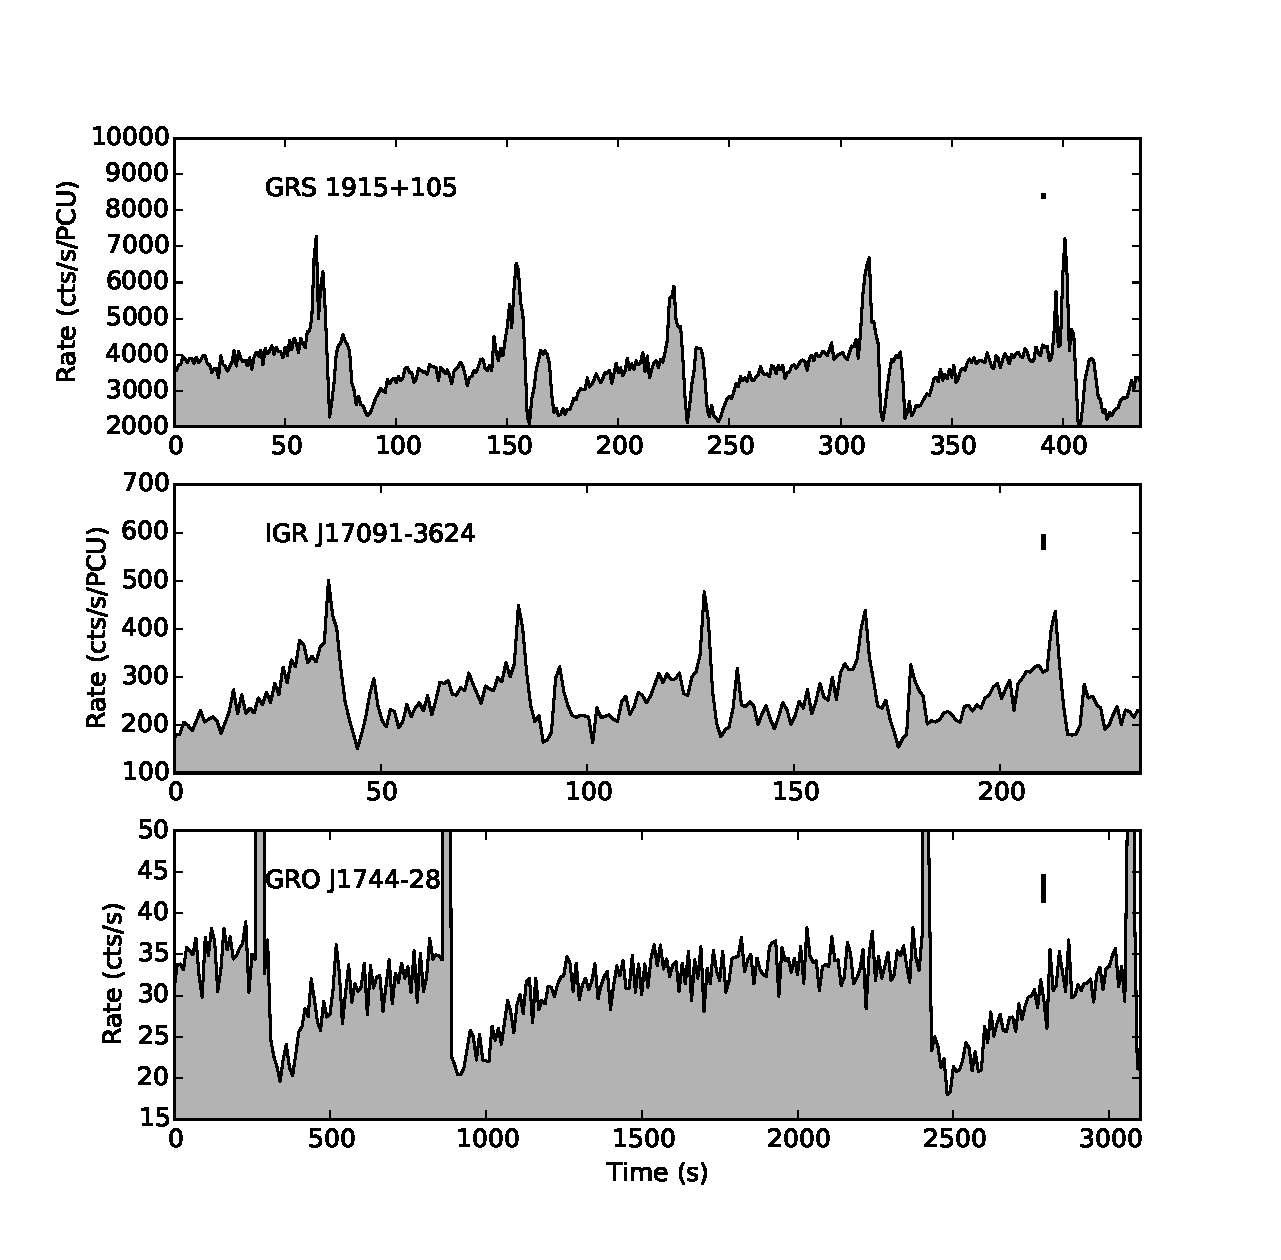
\includegraphics[width=.9\linewidth, trim= 0mm 0mm 0mm 0mm,clip]{images/BPco1.eps}
  \caption[Lightcurves from GRS 1915, IGR J17091 and the Bursting Pulsar, showing lightcurves with Normal Burst-like behaviour for each.]{Lightcurves\index{Lightcurve} from GRS 1915\index{GRS 1915+105}, IGR J17091\index{IGR J17091-3624} and the Bursting Pulsar\index{Bursting Pulsar}, each showing heartbeat\indexrho-like variability\index{Variability} over timescales of 10s to 1000s of seconds.  Black bars indicate average error in each case.  GRS 1915 and IGR J17091 data taken from \indexpca\textit{RXTE}/PCA, Bursting Pulsar data taken from \indexchandra\textit{Chandra}.}
  \label{fig:BP_with_IGR1}
\end{figure}

\begin{figure}
  \centering
  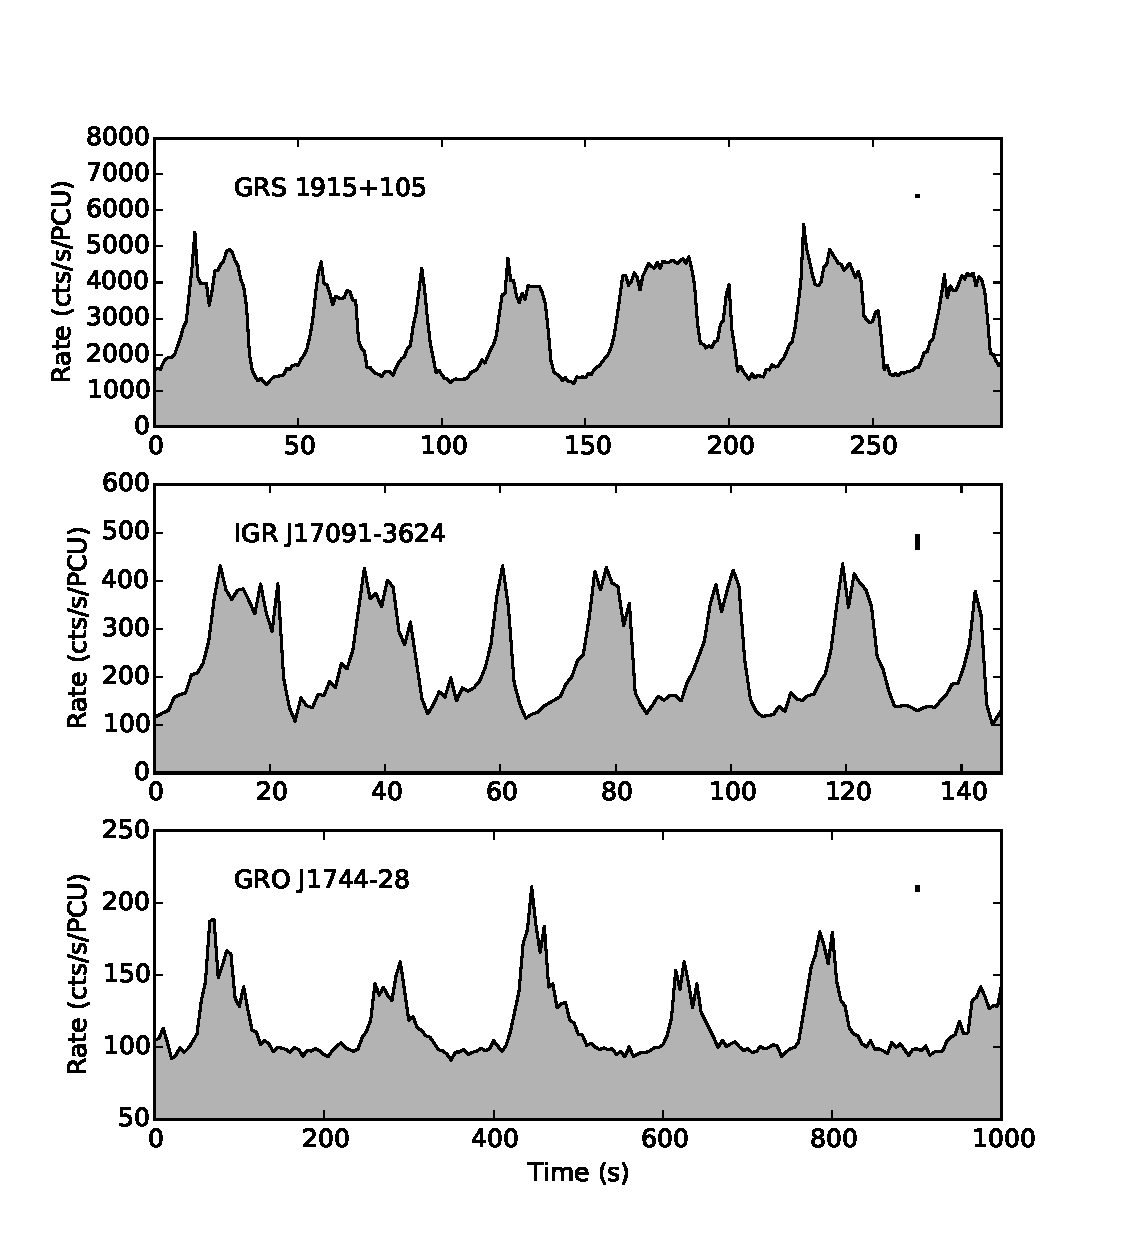
\includegraphics[width=.9\linewidth, trim= 0mm 0mm 0mm 0mm,clip]{images/BPco2.eps}
  \caption[Lightcurves from GRS 1915, IGR J17091 and the Bursting Pulsar, showing lightcurves with Structured Bursting-like behaviour for each.]{Lightcurves\index{Lightcurve} from GRS 1915\index{GRS 1915+105}, IGR J17091\index{IGR J17091-3624} and the Bursting Pulsar\index{Bursting Pulsar}, each showing a Structured Bursting\index{Structured bursting}-like variability over timescales of 10s to 100s of seconds.  Black bars indicate average error in each case.  Data taken from \indexpca\textit{RXTE}/PCA.}
  \label{fig:BP_with_IGR2}
\end{figure}

\begin{itemize}
\item Variability\index{Variability} in IGR J17091\index{IGR J17091-3624} is likely caused by some instability\index{Instability} in the inner, radiation-dominated\index{Radiation pressure} part of its accretion disk\index{Accretion disk}.  The inner region of the disk in the Bursting Pulsar\index{Bursting Pulsar} is dominated by magnetic pressure\index{Magnetic pressure} rather than radiation pressure, leading to different possible instabilities.
\item IGR J17091 can evolve from one variability class\index{Variability class} to another quickly (over timescales of $\lesssim1$ day), whereas Normal Bursts\index{Normal burst} and Minibursts\index{Miniburst} occur continuously in the Bursting Pulsar for many weeks during each outburst\index{Outburst}.
\item IGR J17091 shows complex variability from the peak of each outburst until the time it enters the low/hard state\index{Low/Hard state}, whereas the Bursting Pulsar shows a large gap with no bursts between the end of Normal Bursts and the onset of Mesobursts\index{Mesoburst}.
\item All complex variability in IGR J17091 occurs over a relatively narrow range of luminosities (a factor of $\sim3$, see e.g. Figure \ref{fig:WhereCls}).  Bursting in the Bursting Pulsar occurs at luminosities spanning more than an order of magnitude.
\item All complex variability in IGR J17091 occurs during the main high-soft portion\index{High/Soft state} of its outbursts, whereas Mesobursts and Structured Bursting are seen during rebrightening\index{Re-flare} events in the Bursting Pulsar.
\end{itemize}

Because of these differences, it is unlikely that Burst Classes in the Bursting Pulsar\index{Bursting Pulsar} can be considered as being generated by the exact same phenomenon as variability classes\index{Variability class} in IGR J17091\index{IGR J17091-3624}.  Some of the apparent similarities between the phenomena could instead be explained by phenomenological limit cycles common to both.  For example, if both Class IV\indexiv\ variability and Normal Bursts\index{Normal burst} involve the filling and depletion of a portion of the inner part of the accretion disk\index{Accretion disk}, then it is to be expected that the flares\index{Flare} in both types of variability\index{Variability} have similar morphologies.

\subsection{Structured Bursting}

\par Structured Bursting\index{Structured bursting} in the Bursting Pulsar\index{Bursting Pulsar} on its own can also be compared with the variability classes\index{Variability class} observed in IGR J17091\index{IGR J17091-3624}.  As discussed in Section \ref{sec:struc_var}, and shown in Figure \ref{fig:Types_Struc}, Structured Bursting is a highly variable phenomenon.  Like variability in IGR J17091, Structured Bursting in the Bursting Pulsar consists of flares\index{Flare}, flat-bottomed dips\index{Dip} in flux and periods of seemingly unstructured noise.  As such, an alternative hypothesis to the `hiccup'\index{Hiccup accretion} scenario presented in Chapter \ref{ch:BPletter} is that Structured Bursting is an example of GRS 1915\index{GRS 1915+105}-like variability manifesting in a neutron star\index{Neutron star} LMXB\index{X-ray binary!Low mass}.
\par There are a number of problems with simply equating Structured Bursting\index{Structured bursting} with GRS 1915\index{GRS 1915+105}-like variability classes\index{Variability class}.  Variability in GRS 1915 and IGR J17091\index{IGR J17091-3624} shows hysteresis\index{Hysteresis} in hardness-intensity diagrams\index{Hardness-intensity diagram}, indicating a finite lag\index{Hard lag} between hard and soft emission from the source.  However no such hysteresis exists in Structured Bursting from the Bursting Pulsar\index{Bursting Pulsar}: as we show in Figure \ref{fig:HR}, hardness\index{Colour} and intensity simply correlate during periods of Structured Bursting.  In addition to this, the source intensities involved in GRS 1915-like variability and Structured Bursting are very different; GRS 1915 is a near-Eddington\index{Eddington limit} source, but Structured Bursting in the Bursting Pulsar occurs at a luminosity no greater than 0.5\% of its Eddington Luminosity.
\par If however Structured Bursting\index{Structured bursting} and GRS 1915\index{GRS 1915+105}-like variability\index{Variability} are the same phenomenon, then these issues may be resolved in a number of ways.  While the hard lag\index{Hard lag} in GRS 1915 is positive in every variability class\index{Variability class}, I find that its sign can vary in different variability classes in IGR J17091.  Therefore, it is feasible to imagine a GRS 1915-like system in which this lag is always close to zero, resulting in a simple correlation between rate and hardness in a HID\index{Hardness-intensity diagram} rather than a hysteretic\index{Hysteresis} loop.  Notably, the GRS 1915-like lightcurves\index{Lightcurve} reported from the Rapid Burster\index{Rapid Burster} \citep{Bagnoli_RB} also show no hysteretic loops.
\par The apparent different luminosity regimes of GRS 1915\index{GRS 1915+105} and the Bursting Pulsar\index{Bursting Pulsar} can be resolved if GRS 1915\index{GRS 1915+105}-like variability\index{Variability} does not require near-Eddington\index{Eddington limit} accretion.  I discuss this possibility in Section \ref{sec:criteria}.  The Rapid Burster\index{Rapid Burster} is known to accrete\index{Accretion rate} at $\sim20$\% of its Eddington Limit, and I find that IGR J17091\index{IGR J17091-3624} likely accretes at 5--33\% of its Eddington Limit (Section \ref{sec:newmass}), so these systems set possible precedents for GRS 1915-like variability in systems which are not near-Eddington limited.
\par To further investigate the similarities between GRS 1915-like\index{GRS 1915+105} variability\index{Variability} and Structured Bursting\index{Structured bursting}, the natural next step would be to perform phase-resolved spectroscopy\index{Spectroscopy!Phase-resolved} on Structured Bursting data.  Archival data of Structured Bursting from the Bursting Pulsar\index{Bursting Pulsar} only exists from the 1996 and 1997 outbursts\index{Outburst} of the source, as no observations were taken during the latter stages of its outbursts in 2014 or 2017.  The Bursting Pulsar is a faint source during periods of Structured Bursting, and is in a crowded region of the sky populated by many other X-ray sources, and such a study is difficult to perform on data from instruments launched before 1996.  As such, it remains unclear whether Structured Bursting\index{Structured bursting} is a neutron star\index{Neutron star} manifestation of GRS 1915\index{GRS 1915+105}-like variability\index{Variability} or whether it is a manifestation of `hiccup'\index{Hiccup accretion} accretion as I suggest in Chapter \ref{ch:BPletter}.

\section{Future Research}

\par A number of recently-launched and planned satellites have sensitivities, collecting areas and energy resolutions which exceed those of the instruments I use in this study.  For example, the currently operational \textit{Neutron Star Interior Composition Explorer} (\textit{NICER}, \citealp{Gendreau_Nicer}\index{NICER@\textit{NICER}}) has a 0.5--10\,keV X-ray sensitivity around 30 times greater than that of \textit{RXTE}\indexrxte , with an energy resolution comparable to \textit{XMM-Newton} and \textit{Chandra}\indexxmm\indexchandra.  The European Advanced Telescope for High Energy Astrophysics (\textit{ATHENA}, \citealp{Johnson_Athena}\index{ATHENA@\textit{ATHENA}}), planned for launch in the 2030s, is expected to have a sensitivity around 2 orders of magnitude greater than \textit{XMM-Newton} or \textit{Chandra}.  This generation of highly sensitive instruments will allow us to perform phase-resolved spectroscopy\index{Spectroscopy!Phase-resolved} of variability\index{Variability} from fainter objects, such as IGR J17091\index{IGR J17091-3624} and the Bursting Pulsar\index{Bursting Pulsar} during periods of Structured Bursting\index{Structured bursting}.
\par A phase-reolved spectroscopic\index{Spectroscopy!Phase-resolved} study of the variability classes\index{Variability class} in IGR J17091\index{IGR J17091-3624} will allow us to identify the physical changes in the accretion disk\index{Accretion disk} that occur during each class.  This study will be able to be compared to the phase-resolved spectral study of GRS 1915\index{GRS 1915+105} by \citet{Neilsen_GRSModel}, allowing us to further understand the similarities and differences between these two systems.
\par Phase-resolved spectral studies will also be possible to perform on the fainter classes of bursting\index{Burst} seen in the Bursting Pulsar\index{Bursting Pulsar}.  These will allow us to understand the physical mechanisms underlying each class of burst, in particular identifying which bursts if any are a result of thermonuclear burning\index{Thermonuclear burning} on the surface of the neutron star\index{Neutron star}.  This information will allow us to better understand whether bursting in the Bursting Pulsar is a manifestation of the same instabilities\index{Instability} seen in GRS 1915\index{GRS 1915+105} and IGR J17091\index{IGR J17091-3624}, and will allow us to understand where all of these systems fit in a picture of accretion disk\index{Accretion disk} instability as a whole.